

\documentclass[12pt]{article} 
\usepackage[utf8]{inputenc} % set input encoding (not needed with XeLaTeX)
\usepackage{cite}
\usepackage{geometry} \geometry{a4paper} 
\usepackage{graphicx} 
% \usepackage[parfill]{parskip} 
\setlength{\parskip}{1em}
\begin{document}
\begin{titlepage}
	\newcommand{\HRule}{\rule{\linewidth}{1mm}} % Defines a new command for the horizontal lines, change thickness here
	\center % Center everything on the page
	%----------------------------------------------------------------------------------------
	%	H\begin{aligned}
	%----------------------------------------------------------------------------------------
	
\includegraphics[scale=0.5]{logo.jpg}\\[1cm] % Include a department/university logo - this will require the graphicx package
	\textsc{\LARGE Tribhuvan University, }\\[0.4cm] % Name of your university/college
	\textsc{\Large Pulchowk Campus,}\\[0.4cm] % Major heading such as course name
	\textsc{\large Pulchowk,Lalitpur}\\[0.4cm] % Minor heading such as course title
	%----------------------------------------------------------------------------------------
	%	TITLE SECTION
	%----------------------------------------------------------------------------------------
	\HRule \\[0.4cm]
	{ \large \bfseries Efficiency Enhancement of Wireless Charging System \\[0.3cm] for EV in Static and Dynamic Mode} \\[0.4cm] % Title of your document
	\HRule \\[1.5cm]

	%----------------------------------------------------------------------------------------
	%	AUTHOR SECTION
	%----------------------------------------------------------------------------------------

	\begin{minipage}{0.4\textwidth}
		\begin{flushleft} 
			\emph{Submitted by:}\\
			Anjil Adhikari, (073 BEL 307)\\
			Praveen Kushwaha,(073 BEL 328)\\
			Rabin Dhamala, (073 BEL 329)\\
			Rajib Bijukchhe,(073 BEL 330)\\
		\end{flushleft}
	\end{minipage}
	~	
	\begin{minipage}{0.5\textwidth}
		\begin{flushright} 
			\emph{Submitted to:} \\
			Department of Electrical Engineering, \\
			Pulchowk Campus
		\end{flushright}
	\end{minipage}\\[2cm]

	% If you don't want a supervisor, uncomment the two lines below and remove the section above
	%\Large \emph{Author:}\\
	%John \textsc{Smith}\\[3cm] % Your name

	%----------------------------------------------------------------------------------------
	%	DATE SECTION
	%----------------------------------------------------------------------------------------

	{\large \today}\\[2cm] % Date, change the \today to a set date if you want to be precise

	%----------------------------------------------------------------------------------------
	%	LOGO SECTION
	%----------------------------------------------------------------------------------------


	%----------------------------------------------------------------------------------------

	\vfill % Fill the rest of the page with whitespace
\end{titlepage}


\tableofcontents
\newpage

\renewcommand{\baselinestretch}{1.5}
\section{Terms}
\textit{Wireless Charging Systems (WCS), 
	Wireless Power Transmission Systems (WPTS), 
	Resonant Inductive Coupling (RIC),
	Electric Vehicles (EV), 
	Maximum Power Point Tracking(MPPT),
	Wireless power transfer (WPT),
	Proportional Integral(PI),
	Proportional Integral Derivative(PID),
	Battery Management Systems (BMS),
Wireless Electric Vehicle Charging System (WEVCS)}


\section{Objective}
\textit{To improve power transfer efficiency of wireless charging system for EVs in static and dynamic mode}

\section{Motivation}
In recent decades, there have been significant developments and breakthroughs in technology. The use of a variety of autonomous electronics devices; such as mobile phones, laptops, tablets and home appliances has significantly increased due to consumer demands. Such electronics contain on-board energy storage modules in the form of lithium based batteries. These batteries have normally been charged by conventional battery chargers through physical contacts. This form of connection increases the risk of short circuits; either by water or foreign objects crossing the contacts, or due to damaged connectors. In addition, different electronic devices have different power ratings as well as a variety of standardized chargers. Standardised chargers create inconvenience to the users when they travel to another country. Moreover, when such electronic devices are upgraded or replaced, the chargers also need replacing even though they may still be in good working order. These unused devices end up in landfill because of improper recycling. This is known as electronic waste (E-Waste). Worldwide 20 to 50 million tonnes of E-Waste is annually generated.

In order to reduce the usage of high priced fossil fuels, electrified transportation requires the set-up of a wide variety of charging networks to create user-friendly environments and to tackle green-house and fuel price hikes. To compete with gasoline-powered cars, EVs are required to have a long travelling range with an efficient refuel capacity. These features can only be achieved by installing a larger battery bank with continual charging facilities. However, a larger battery bank increases the overall price of EVs and requires additional charging time. Such limitations are the biggest hurdles in making EVs a reliable transportation alternative. WCS can provide a common charging platform for most electronic devices so different electronic products do not require separate standardised chargers to charge their batteries. Moreover, it can help to reduce the battery storage requirements by providing a continuous dynamic charging facility wirelessly. This technology can reduce toxic and non-biodegradable hazardous E-waste by establishing a common charging platform for all electronic products. %cite

In order to tackle these issues, Wireless Charging Systems(WCS) are one of the up and coming technologies which have the potential to provide contactless charging facilities in low, medium and high power consumer electronic products. WCS technology can offer \textbf{safe, secure ,reliable} and \textbf{user friendly} charging techniques that are environmentally sound. 
\section{Introduction}
In the 21st century, wireless power transmissionsystems (WPTS) are considered to be advanced technologies for numerous applications
such as mobile devices, home appliances, and medical implants in the areas of low and medium voltage electronics devices, by the utilisation of two fundamental important mechanisms: inductive coupling and strong electromagnetic resonant coupling %[15].

Firstly, the inductive coupling method with resonant case was identified and used in the experiment by Nikola Tesla in 1914.  This method is also known as Resonant Inductive Coupling (RIC). His idea was to transfer power over a long distance globally. Radiative transfer is suitable for transferring data and other information over the air, over a long distance, by using antennas. However, when it comes to power transfer, it is very difficult to use this method because most of the energy is lost in the air because of the omni-directional transmission. Otherwise, it requires a line of sight and an advanced tracking system at the receiver side. Inductive coupling is an immersing method to transfer power wirelessly in the power ranges between mill watts and some kilowatts.
However, when it comes to efficiency, it decreases significantly with increasing distance between the primary and secondary circuit.The problem or limitation associated with WCS is that they can only be utilised when the vehicle is parked or in stationary modes such as in car parks, garages or at traffic signals . In addition, stationary WCS have some challenges such as limited power transfer, bulky structures,shorter range and higher efficiency. 

In order to improve both areas (range and sufficient volume of battery storage), a dynamic mode of operation of the WCS for EVs has been researched. Inductive charging of electric vehicle at high power levels while in motion is referred to as dynamic charging. If a car was able to be charged while it was being driven, then this would solve the problem of limited range and enable vehicles to travel for potentially unlimited distances. The idea is that a coil on the bottom of a car could receive electricity from coils that are connected to an electric current that is emnedded in the road. However, before a dynamic WCS becomes more widely accepted, it has to overcome two main hurdles: a large air gap and coil misalignment. As the distance between the two coils is getting larger, the voltage at the receiver end of the transmission reduces. To compensate for the variation of the voltage, different control methods( a three-level PI controller, fuzzy and neuro fuzzy conntroller, MPPT control) are employed to improve system efficiency. 

A simple block diagram implementation of wireless charging system is shown below in figure \ref{fig:scheme}:
\begin{figure}[h!]
	\centering
	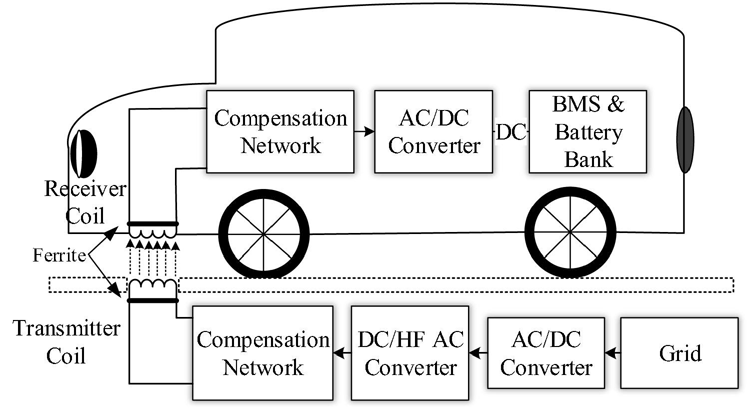
\includegraphics[scale=0.5]{image1.jpg}
	\caption{Schematic of Wireless Charging System}
	\label{fig:scheme}
\end{figure}
\newpage
\section{Literature}
Wireless electric vehicle charging techniques have been popular for some time now due to their
safety, convenience and efficiency. There are several ways to increase the WPT efficiency of a system.
First is by the proposed Series-Series (SS) resonant compensation topology alongside the design of
radio frequency feedback (Tan, 2017). This proposed model was experimented and tested with a
500W laboratory prototype and it was found that the efficiency was above 90\%, an air gap was 15
cm, distance was 10cm and over an operating input voltage of 120VAC (Tan, 2017). The second
method used to enhance WPT efficiency is by varying the operating frequency ranging from 81.38-90 kHz, 
the duty ratio and input voltage respectively (Ravikiran, 2017). The other technique employed
was by finding a reference voltage in the secondary side using the simultaneous estimation of the
secondary side's mutual inductance and a voltage at the primary side (Hata, 2016). In addition, the
compensation topologies play a key role in the power transfer efficiency, therefore, this paper gives a
detailed comparison between the SS and PS compensation topologies (Ravikiran, 2017). Simulation
results show that the PS topology is good for power applications of medium range. This paper uses
secondary side LCC impedance matching circuit under a rectifier load to enhance the maximum
efficiency transferred (Liao, 2017).

To keep up with the pace of battery capacities, it is essential to increase the rate at which an
electric vehicle battery is wirelessly charged. One of the ways of increasing battery performance is
by designing the coupling factor of the coil system appropriately and ensuring that the rate of
displacement is large (Klaus, 2017). Another way to increase the power transfer system of an electric
vehicle is to use two extra coils in between the transmitter and the receiver coils with experimental
verification with a 6.6KW circuit (Tran, 2018). This results in an efficiency of 97.08\% for 3.4KW.
For different challenges associated with WPT to be addressed, this paper proposed employing an
20 improved floor surface for shielding the transmitting coil area, high-frequency switches with large
bandgap switches and polygon iron core (Mahmud, 2017). These components help to improve the
system's efficiency.

Subsequently, a wireless power charging system requires a constant current flow and output
voltage alongside a maximum efficiency. This leads to the design of a control based maximum
efficiency tracking system that controls the transmitter current based on the information the receiver
receives via Bluetooth (Yeo, 2017). This gives a constant output voltage and constant current flow
with increased efficiency in the WPT system. A fixed voltage source and fixed current load are
modeled, analyzed and verified experimentally to increase the wireless power charging system's 
efficiency (Zhang, 2017). The voltage on the receiving coil in a wireless power transfer depends on the
distance between two coils. This paper implements a proportional integral controller at the receiver
side of the wireless power transfer to eliminate the variation of voltage for a varied distance between
the two coils (Yeo, 2017). \cite{a2019}

\section{Methodology}
\subsection{For static mode}
\begin{enumerate}
	\item The different resonant circuit will be modeled . Simulation results will be carried out showing the effect of parameters such as inductor, capacitor, load and coupling coefficient on efficiency. 
	\item 3D modeling of transmitting and receiving coil using ANSYS Maxwell. 
	\item Design of system circuit in ANSYS Simplorer. 
	\item Design of complete system of a magnetic resonance WPT in Maxwell. 
	\item Comparing Magnetic Induction Power Transfer with Magnetic Resonance Method. 
\end{enumerate}

\subsection{For dynamic mode}
\begin{enumerate}
	\item Design of three-level cascaded PI controller  to eliminate the variation of voltage because of varied spacing existing between both coils.
	\item Design of fuzzy logic and neuro-fuzzy controller.
	\item Design of three-level cascaded MPPT controller. 
		The design of dynamic mode controllers will be done using Matlab Simulink. 
\end{enumerate}
\newpage
\section{Operating Theory}
\begin{figure}[h]
	\centering
	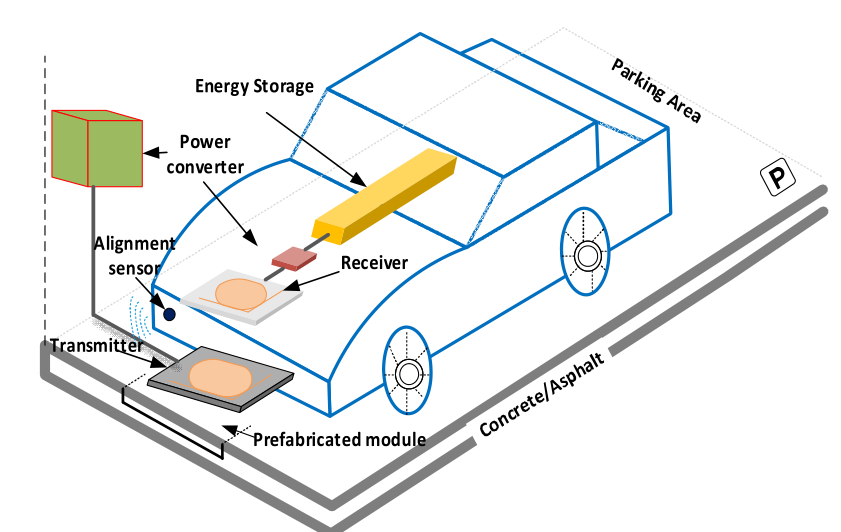
\includegraphics[scale =0.75]{static.png}
	\caption{Wireless Charging model of EV}
	\label{fig:WEV}
\end{figure}
Figure \ref{fig:WEV} shows the basic arrangement of WEVCS. The primary coil is installed underneath in the road or ground with additional power converters and circuitry. The receiver coil, or secondary coil, is normally installed underneath of the EVs front, back
or center. The receiving energy is converted from AC to DC using the power converter and is transferred to the battery bank. In order to avoid any safety issues, power control and battery management systems (BMS) are fitted with a wireless communication network to receive any feedback from the primary side. The charging time depends on the source power level, charging pad sizes, and air gap distance between the two windings. The average distance between lightweight duty vehicles is approximately 150 mm - 300 mm. Static WEVCS can be installed in parking areas, car parks, homes, commercial buildings, shopping centres. \cite{pl2018}
\begin{figure}[h]
	\centering
	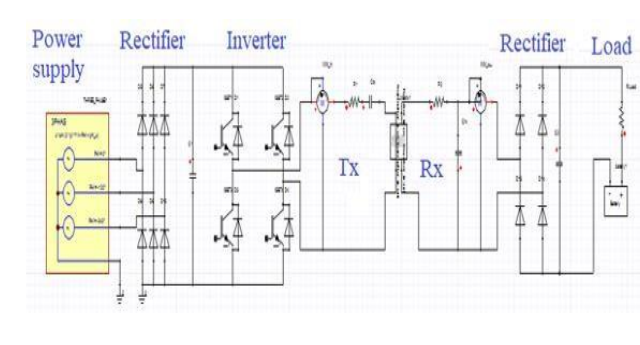
\includegraphics{circuit.png}
	\caption{circuit diagram of electric wireless system}
	\label{fig:ckt}
\end{figure}
  %block diagram of static
 \newpage 
  
\bibliographystyle{plain}
\bibliography{main}
\end{document}
